\documentclass[12pt]{article}

%%%%%%%%%%%%%%%%%%%%%%%%%%%%%%%%%%%%%%%%%%%%%%%%%%%%
% Preamble:
%%%%%%%%%%%%%%%%%%%%%%%%%%%%%%%%%%%%%%%%%%%%%%%%%%%%
% Typical Packages:
\usepackage[utf8]{inputenc}
\usepackage{fullpage}
\usepackage{amsfonts}
\usepackage{amsmath}
\usepackage{amsthm}
\usepackage{amssymb}
\usepackage{mathrsfs}
\usepackage{graphicx}
\usepackage{color}
\usepackage{palatino}
\usepackage{url}
\usepackage{multicol}
\usepackage{enumerate}
\usepackage{ulem}
\usepackage{tikz}
\usepackage{tipa}
\usepackage{upgreek}
\usepackage{hyperref}
\usepackage{verbatim}
\usepackage{caption}
\usepackage{fancyhdr}

\thispagestyle{empty}

% Fancy Header Package:
\usepackage{fancyhdr}
\setlength{\headheight}{15.2pt}
\pagestyle{fancy}
\setlength\headsep{30pt}
\lhead{Mini-Project 2 Report}
\rhead{Trevor Wylezik}

%%%%%%%%%%%%%%%%%%%%%%%%%%%%%%%%%%%%%%%%%%%%%%%%%%%%
% Title:
%%%%%%%%%%%%%%%%%%%%%%%%%%%%%%%%%%%%%%%%%%%%%%%%%%%%
\title{Mini Project 2 - Interpolation and Curve Fitting}
\author{Trevor Wylezik}
\date{\today}



%%%%%%%%%%%%%%%%%%%%%%%%%%%%%%%%%%%%%%%%%%%%%%%%%%%%
% Start Document:
%%%%%%%%%%%%%%%%%%%%%%%%%%%%%%%%%%%%%%%%%%%%%%%%%%%%
\begin{document}

\maketitle

\abstract
{\noindent
In 2020, the world was struck with COVID-19, a highly contagious virus. Even though this was a fatal virus for some, it made for some interesting discoveries in the sciences as we suddenly had one of the most in-depth virus data collections alongside the technological advancements of the twenty-first century. Scientists predicted that we would see the data represent a logistic curve that is typically used to predict population growth (Figure 1). In this report, we will investigate state COVID case data to see if we can extract logistic curves that fit to the data. We will also focus on the delta variant of COVID-19 as it was even more infectious and shows a clear spike in the data. The fitting for this data will be using California data as it is most credible (high population). 
}

\begin{center}
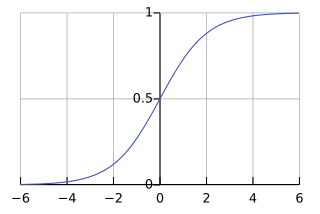
\includegraphics[width = .6\textwidth]{Logistic Curve.png}\\
Figure 1: A generic logistic curve with inflection point $x=0$ and capacity $L=1$. 
\end{center}
\pagebreak


%%%%%%%%%%%%%%%%%%%%%%%%%%%%%%%%%%%%%%%%%
% Introduction Section: 
%%%%%%%%%%%%%%%%%%%%%%%%%%%%%%%%%%%%%%%%%
\section{Introduction}
In this report, we will investigate COVID-19 case data and analyze the behavior with respect to time. In particular, each state has recorded daily data on the number of total covid cases, recoveries, deaths, and other metrics. This report will focus on the COVID-19 cases that follow a logistic curve (Figure 1). This project starts with collecting the COVID-19 data from a known source and cleaning this data in excel. Then, this cleaned data set will be pulled in to python for further analysis with Pennsylvania, California, Texas, Florida, and New York. The curve fitting will be with California data and uses concepts from linear algebra such as linearization, normal equations, and Vandermonde matrices. Next, statistics concepts like the minimization of least squares will be used to model the data and produce legible charts. \\

\noindent This project is organized as follows: In Section 2, we will highlight the problem statement. In section 3, we will go in-depth in to the cleaning of the data set, pulling it in to python, and performing the curve fitting. Section 4 and 5 will be the final results of the project and a discussion about the tool and results. Finally, Section 6 will be conclusions of the project.

\section{Problem Statement}
\noindent The goal of this project is to model data using linear algebra concepts and built in python functions from NumPy, SciPy, and Matplotlib. These will be used to solve both interpolation and linear least squares formulations. \\

%%%%%%%%%%%%%%%%%%%%%%%%%%%%%%%%%%%%%%%%%
% Methodology Section: 
%%%%%%%%%%%%%%%%%%%%%%%%%%%%%%%%%%%%%%%%%
\section{Methodology}
In this section, we will dive in to the data collection/cleaning and model building. 

\subsection{Data Collection and Cleaning}
The data for this project comes from a COVID-19 data repository from the Center for Systems Science and Engineering (CSSE) at Johns Hopkins University. The data is in the format of CSV files for each day of data collected. This was then imported in to one excel file for further investigation. \\

\pagebreak

\noindent At first, the data was messy and had a lot of unnecessary information as seen below. 

\begin{center}
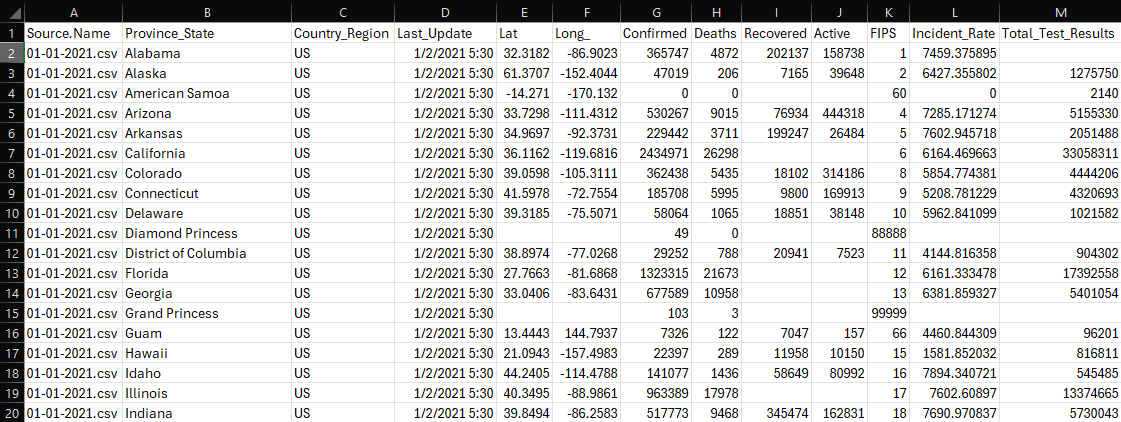
\includegraphics[width = 0.9\textwidth]{Messy data.png} \\
Figure 2: The original excel file with state COVID-19 data (before cleaning).
\end{center}

\noindent This dataset was updated to make it easier to work with. Some of these updates are as follows: removing US territories and cruise ships, changing the date column to be a serial number, removing duplicate rows, removing latitude/longitude and other unnecessary columns. These changes can be seen below.

\begin{center}
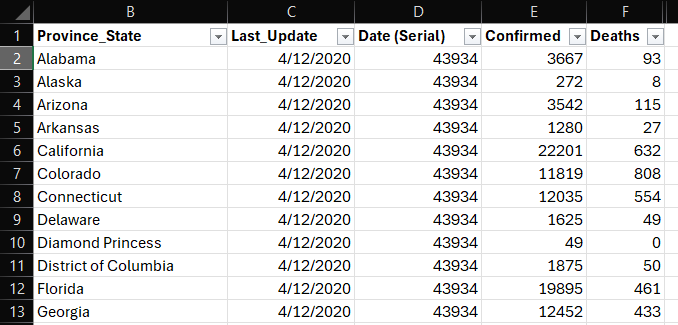
\includegraphics[width = 0.9\textwidth]{clean data.png} \\
Figure 3: Cleaned COVID-19 state data set.
\end{center}

\noindent With a full data set of COVID-19 data that is cleaned easily accessible, we can now pull this data in to python in the next section. \\

\noindent Note: For all of the curve fitting the data has to be normalized to the interval $(0,1)$ and then scaled back up for charting purposes.

\pagebreak

\subsection{Pulling and Organizing Data in Python}
\noindent For the purposes of pulling excel data in to python, Pandas will be the main tool used. We first have to create a data frame and segment the data in to specific states that we want to see.

\begin{center}
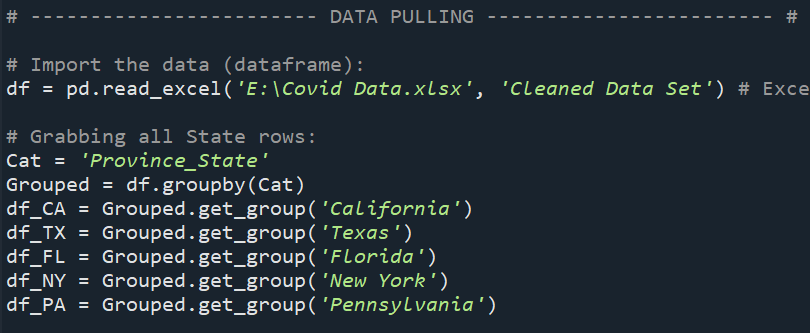
\includegraphics[width = 0.9\textwidth]{data pulling1.png} \\
Figure 4: Pulling an excel file in to Python and grouping rows by states.
\end{center}

\noindent We can now view each state's data and see the waves of COVID-19 spreading rapidly. This was done with Florida, Pennsylvania, New York, and Texas as examples to show the logistic curves.

\begin{Figure}
\begin{center}
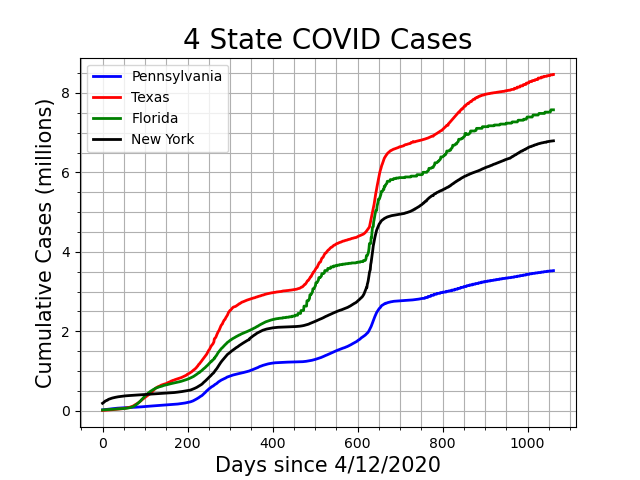
\includegraphics[width = 0.7\textwidth]{4 state data.png} \\
Figure 5: NY, CA, FL, and TX COVID-19 cumulative case data.
\end{center}
\label{5}
\end{Figure}

\pagebreak

\subsection{Linearly Solved Logistic Fit}
\noindent The focus of this fit was to look at a specific time span when the delta variant of COVID-19 was spreading. This variant was less lethal than normal, but was more contagious leading to higher COVID-19 cases. \\

\noindent First, we can look at a generic logistic equation to base our model on:
\[
\displaystyle y=\frac{1}{1+ae^{-bx}} \\
\]
This equation is able to rearranged and expressed linearly as follows:
\[
\begin{array}{rl}
    \implies{} & \displaystyle\frac{1}{1+ae^{-bx}}=y \\ \\
    \implies{} & \displaystyle 1+ae^{-bx}=\frac{1}{y} \\ \\
    \implies{} & \displaystyle ae^{-bx}=\frac{1}{y}-1 \\ \\ 
    \implies{} & \ln{(ae^{-bx})}=\ln{(\frac{1}{y}-1)} \\ \\
    \implies{} & \ln{a}+\ln{e^{-bx}}=\ln{(\frac{1}{y}-1)} \\ \\
    \implies{} & \ln{(a)}+\ln{(e^{-bx})}=\ln{(\frac{1}{y}-1)} \\ \\
    \implies{} & \ln(a) - bx = \ln{(\frac{1}{y}-1)}
\end{array}
\]
This results in the following matrix equation:
\[ \underbrace{
\left[\begin{array}{cc}
1 & -x_{1} \\ \\
1 & -x_{2} \\ \\
\vdots & \vdots \\ \\
1 & -x_{n}
\end{array}\right]}_{\displaystyle A}
\underbrace{\left[\begin{array}{c}
\ln{(a)} \\ \\
b
\end{array}\right]}_{\displaystyle\vec{c}} = 
\underbrace{\left[\begin{array}{c}
\ln{(\frac{1}{y_{1}}-1)} \\ \\
\ln{(\frac{1}{y_{2}}-1)} \\ \\
\vdots \\ \\
\ln{(\frac{1}{y_{n}}-1)}
\end{array}\right]}_{\displaystyle\vec{y}}
\]

\pagebreak

\noindent The normal equation for regression can then be made and solved for $\vec{c}$. \\
\[
\displaystyle\left(A^{T}A\right)\vec{c}=A^{T}\vec{y} \\
\]
Solving the above normal equation with numpy and plotting the generic logistic function with $a$ and $b$ produces the following chart and values:
\[
\text{Logistic Equation: } y=\frac{1}{1+ae^{-bx}} \\
\]
\[
a = 0.6507 \,\text{ and }\, b = 0.1138 \,\text{ (rounded to 2 decimal places)}
\]
\[
R^{2}=0.9846
\]
\begin{center}
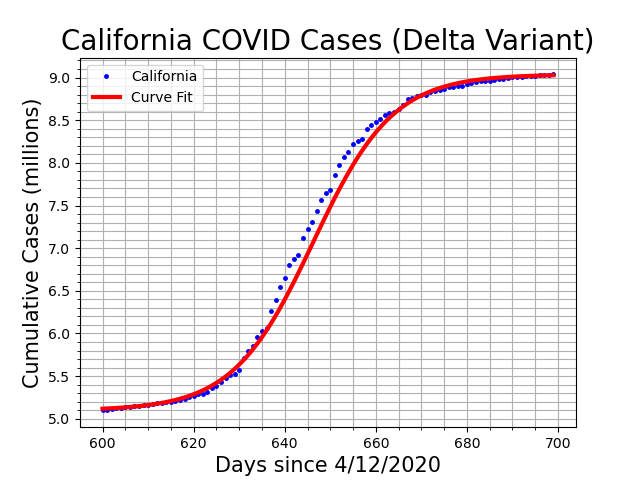
\includegraphics[width = 0.7\textwidth]{california delta.png} \\
Figure 6: California COVID cases between 12/3/2021 and 3/13/2022 (delta variant).
\end{center}

\pagebreak

\subsection{Multiple-Logistic Curve Fit}
The COVID-19 cases seemed to follow a logistic curve, but repeated as COVID-19 infected people in waves. This is difficult to model from the start as the logistic function acts in such a way that it has one inflection point ($x_{0}$), maximum value (carrying capacity $L$), and growth rate ($k$). But, each jump in the COVID-19 case data is not at the same place with the same capacity, and does not have the same growth rate. \\

\noindent One way around this is to add multiple logistic functions together that are all offset from each other. This works since all values are effectively flat at the bottom and top of the curve. It seems like the data has 3 main growth points, so we will look at a multiple-logistic curve fit with 3 jumps.
\[
\displaystyle y = 
\frac{L_{1}}{1+e^{-k_{1}(x-x_{1})}} + 
\frac{L_{2}}{1+e^{-k_{2}(x-x_{1}-x_{2})}} +
\frac{L_{3}}{1+e^{-k_{3}(x-x_{1}-x_{2}-x_{3})}} \\
\]

\noindent In simpler terms, $L_{i}$ is additional the height of the carrying capacity from the section of the curve. $k_{i}$ is the $i^{th}$ curve's growth rate. And $x_{i}$ is the distance from the previous inflection point. After using SciPy's optimize curve fit function, the chart and values were produced: \\
\[
\begin{array}{c}
     L_{1}=0.20518 \qquad L_{2}=0.24404 \qquad L_{3}=0.73664 \\
     k_{1}=0.05945 \qquad k_{2}=0.17356 \qquad k_{3}=0.00452 \\
     x_{1}=250.077 \qquad x_{2}=393.792 \qquad x_{3}=143.726 \\
     R^{2}=0.9984
\end{array}
\]
\begin{center}
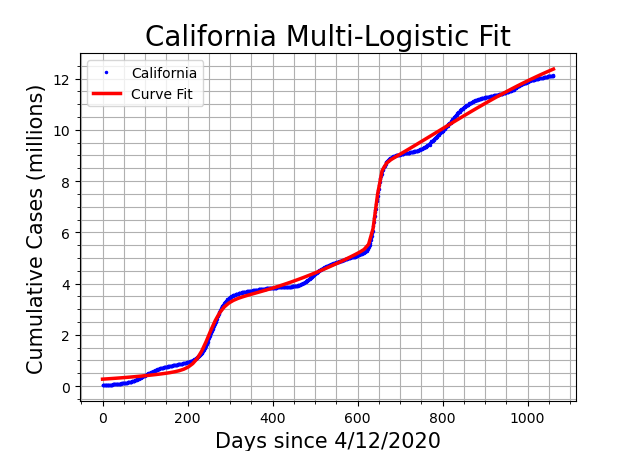
\includegraphics[width = 0.8\textwidth]{multi-logistic fit.png} \\
Figure 7: California COVID cases with a multi-logistic curve fit.
\end{center}

\pagebreak


\section{Results}
We have now been able to analyze COVID-19 data at the state level and show that it follows a classic logistic curve. This is due to the high $R^{2}$ values that represent the proportion of error due to the fit (which is related to minimal error). 

\section{Discussion}
This project had many intricacies in the coding process that took a substantial amount of time. For example, the California case data is in the millions over a thousand day time period. This caused the curve fitting to struggle as it had to hit such high points in the data. \\

\noindent A way around this was by normalizing the data to make everything fit in between $(0,1)$ (not inclusive). This caused the data to be easier to work with and then was able to scaled back up to its original size. Some values like $L_{i}$ and $k_{i}$ seem very small in this respect, and that is the reason why.

\section{Conclusion}
In this project, interpolation and curve fitting was used to find functions that represent COVID-19 data. This was done by first collecting and cleaning data, then pulling that data in to python to run least squares curve fitting, and finally producing optimized parameter values and legible charts. \\

\section{Resources}
For this project, the data was sourced from The Center for Systems Science and Engineering (CSSE) at Johns Hopkins University following hyperlink: \\

\noindent \href{https://github.com/CSSEGISandData/COVID-19}{COVID-19 Data by state} \\




\end{document}